\begin{figure*}[!h]
\begin{subfigure}{0.195\linewidth}
\centering
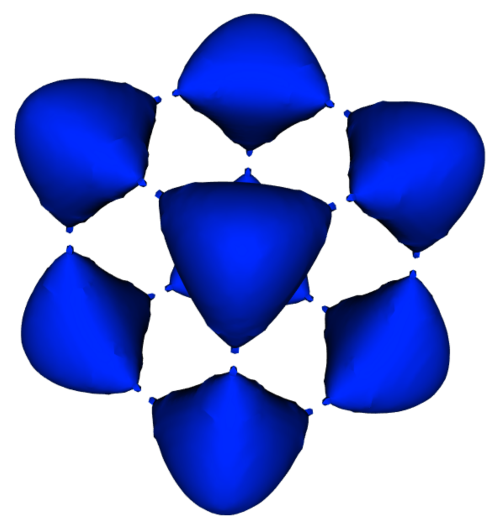
\includegraphics[width=0.8\linewidth]{Images/Tangle/gt.pdf}
\vspace{-2mm}
\caption{Ground truth, $isoval=62$}
\label{fig:tangle_gt}
\end{subfigure}
\begin{subfigure}{0.195\linewidth}
\centering
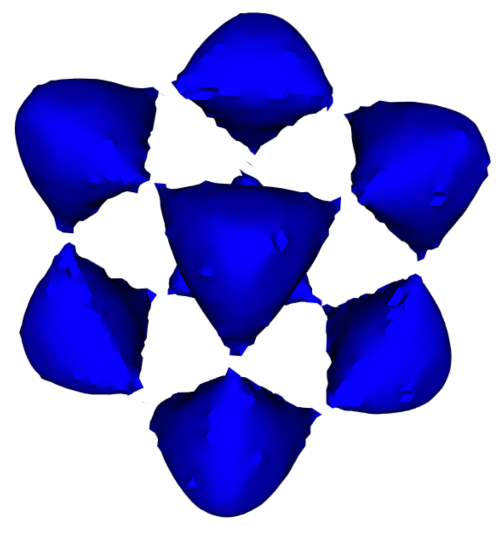
\includegraphics[width=0.8\linewidth]{Images/Tangle/zls.pdf}
\vspace{-2mm}
\caption{$ZLS_{T}$}
\label{fig:tangle_zls}
\end{subfigure}
\begin{subfigure}{0.195\linewidth}
\centering

\includegraphics[width=0.8\linewidth]{Images/Tangle/fls.pdf}
\vspace{-2mm}
\caption{$ZLS_{T}$ + $FLS_{T,2}$}
\label{fig:tangle_fls}
\end{subfigure}
\begin{subfigure}{0.195\linewidth}
\centering
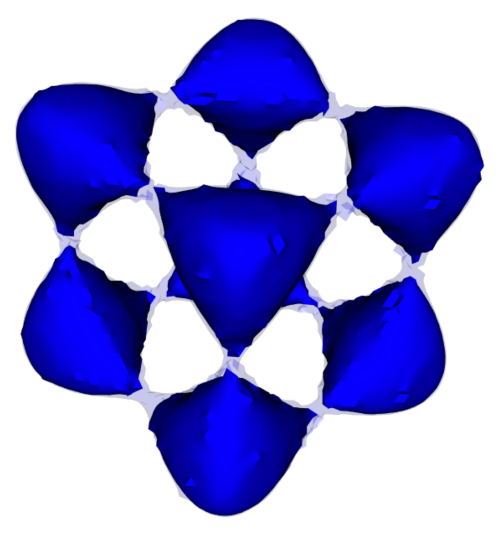
\includegraphics[width=0.8\linewidth]{Images/Tangle/fcls_68.pdf}
\vspace{-2mm}
\caption{$ZLS_{T}$ + $FCLS_{T,68\%}$}
\label{fig:tangle_fcls_68}
\end{subfigure}
\begin{subfigure}{0.195\linewidth}
\centering
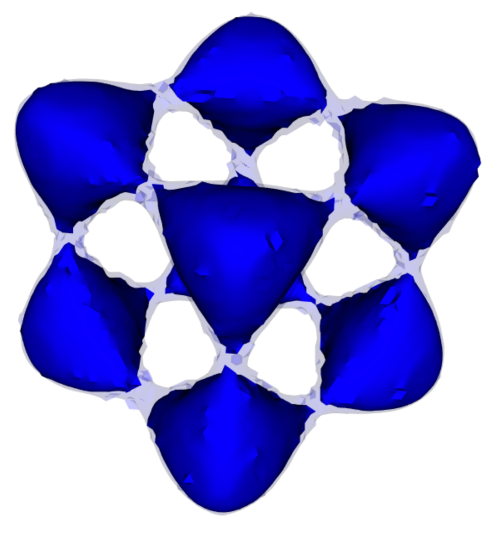
\includegraphics[width=0.8\linewidth]{Images/Tangle/fcls_95.pdf}
\vspace{-2mm}
\caption{$ZLS_{T}$ + $FCLS_{T,95\%}$}
\label{fig:tangle_fcls_95}
\end{subfigure}
\vspace{-2mm}
\caption{Visualization of sensitivity of the tangle function near values that form links between the multiple blobs. We use $T=[0,62]$.}
\vspace{-2mm}
\label{fig:tangle}
\end{figure*}

We demonstrate the use of feature confidence level-sets using five data sets.
%
Specifically, we consider an analytical tangle function~\cite{knoll2009fast}, an EF-5 Tornado~\cite{atmos10100578}, the ethanediol molecule~\cite{}, Red Sea and Gulf of Aden~(RSGOA) eddy ensemble~\cite{sanikommu2020impact} and Earth's mantel convection~\cite{shahnas2017mid} data.
%
We defined traits based on prior knowledge of features of interest in the data.
%
While our study demonstrates feature confidence level-sets for univariate and bivariate data, the approach can be applied to higher dimensions.
%
For this study, each attribute is represented using a $mean$ and $SD$ field. 
%
For the RSGOA data set, we computed $mean$ and $SD$ fields across ensemble members. 
%
For every other data set, we synthetically compute $SD$ at each grid point by sampling the local neighborhood.
%
For each data set, we visualized the $ZLS_{T}$ individually, and augment it with a semi-opaque, single feature level-set $FLS_{T,K}$ for some level $K$, or a feature confidence level-set $FCLS_{T,C}$ for some confidence $C$ (and level $\epsilon$).
%

For all data sets considered, as expected we found $FLS_{T,K}$ has the shortcoming of discernability.
%
The $FLS_{T,K}$ level-set typically formed a ``shell'' like structure.
%
In constrast, the shape of the $FCLS_{T,C}$ level-set corresponded to the uncertainty of the data in the spatial domain.
%
For example, for the tangle function where uncertainty is higher near the links between the blobs, comparing Figures~\ref{fig:tangle_fcls_68} and~\ref{fig:tangle_fcls_95} we found the $FCLS_{T,C}$ envelope expanded between the links in response to increasing the value of $C$, but not significantly on the exterior of the blob itself.

In comparison to $FLS_{T,K}$, for uncertain multivariate data, by leveraging the information pertaining to field distribution~($mean$, $SD$), $FCLS_{T,C}$ provided improved secondary structure visualization.
%
For example, we observed additional weaker tornado vortices in Figure~\ref{fig:tornado_fcls}, improved molecular structure information for the ethanediol covalent and non-covalent bonds in Figure~\ref{fig:ethanediol_fcls}, regions with anticyclonic and cyclonic eddies in Figure~\ref{fig:rse_fcls}, and the interaction of flow patterns in the mantel data set in Figure~\ref{fig:mantel_fcls}.
%
Importantly, for the traits selected, the secondary structures produced using $FCLS_{T,C}$ did not overlap one another.
%
In contrast, for the same traits, $FLS_{T,K}$ resulted in overlapping and occluding level-sets~(see Figure~\ref{fig:rse_fls}).
%
We provide supplementary visualizations and comparisons in the additional material. 
 
\begin{figure*}[!h]
\begin{subfigure}{0.20\linewidth}
\centering
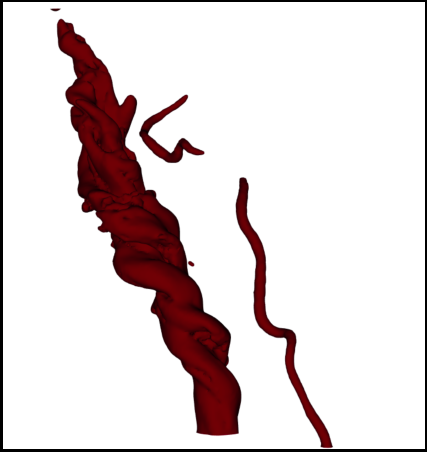
\includegraphics[width=0.9\linewidth]{Images/Tornado/zls.pdf}
\vspace{-1mm}
\caption{$ZLS_{T}$}
\label{fig:tornado_zls}
\end{subfigure}
\begin{subfigure}{0.20\linewidth}
\centering
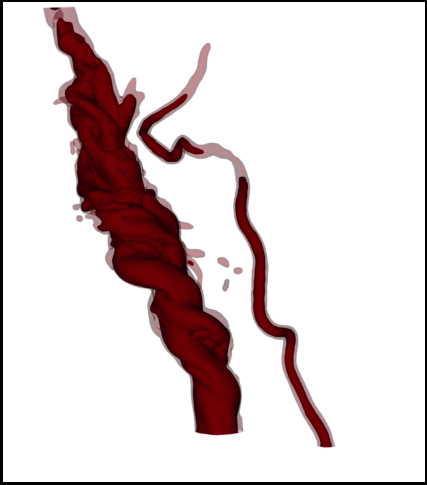
\includegraphics[width=0.9\linewidth]{Images/Tornado/fcls_50.pdf}
\vspace{-1mm}
\caption{+ $FCLS_{T,50\%}$}
\label{fig:tornado_fls}
\end{subfigure}
\begin{subfigure}{0.20\linewidth}
\centering
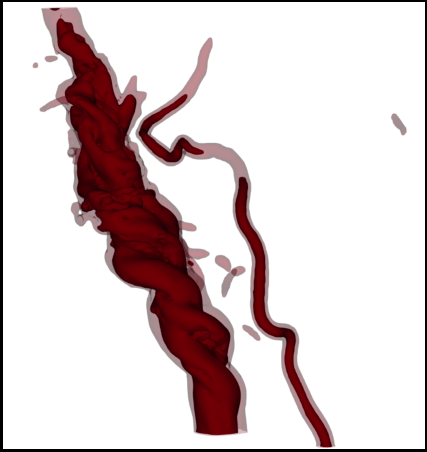
\includegraphics[width=0.9\linewidth]{Images/Tornado/fcls_68.pdf}
\vspace{-1mm}
\caption{+ $FCLS_{T,68\%}$}
\label{fig:tornado_fls}
\end{subfigure}
\begin{subfigure}{0.20\linewidth}
\centering
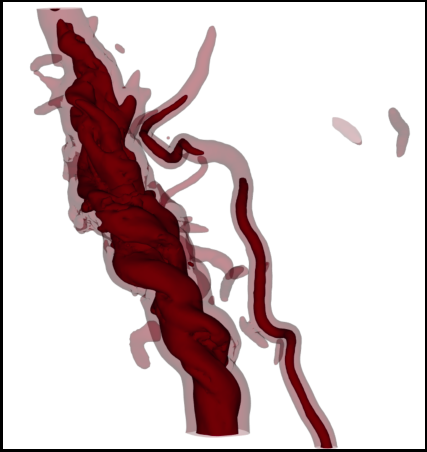
\includegraphics[width=0.9\linewidth]{Images/Tornado/fcls_95.pdf}
\vspace{-1mm}
\caption{+ $FCLS_{T,95\%}$}
\label{fig:tornado_fcls}
\end{subfigure}
\hfill
\begin{subfigure}{0.17\linewidth}
\centering
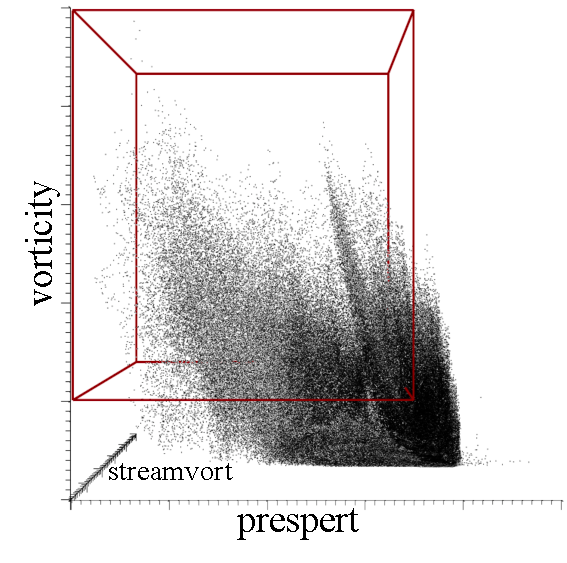
\includegraphics[width=\linewidth]{Images/Tornado/scatterplot3d.pdf}
\vspace{-4mm}
\caption{3D scatterplot of $\mathcal{A}$ and $T$ (red cuboid).} 
\label{fig:tornado_scatterplot}
\end{subfigure}
%\vspace{-2mm}
\caption{Visualization of EF-5 tornado vortices using vorticity, prespert and streamvort attributes. As in Figure~\ref{fig:tangle}, $FCLS_{T,C}$ formed wider envelopes as $C$ increased. Importantly, $FCLS_{T,C}$ visualized vortical structures of interest in the vicinity of the primary tornado vortex.}
%\vspace{-1mm}
\label{fig:tornado}
\end{figure*}

\begin{figure*}[h]
\begin{subfigure}{0.18\linewidth}
\centering
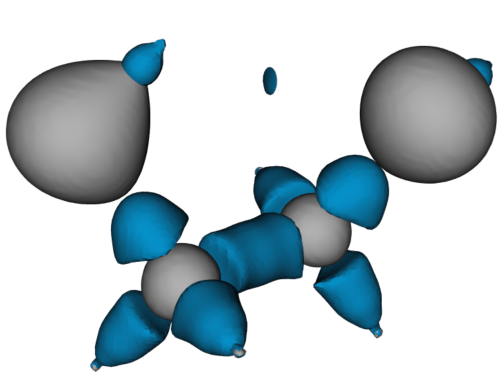
\includegraphics[width=\linewidth]{Images/EthaneDiol/gt.pdf}
\caption{$Rho_{isoval}=1.57$ (gray),\\ $s_{isoval}=-0.575$ (light blue)}
\label{}
\end{subfigure}
\begin{subfigure}{0.18\linewidth}
\centering
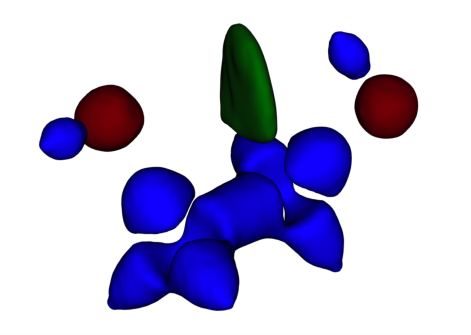
\includegraphics[width=\linewidth]{Images/EthaneDiol/zls_3.pdf}
\caption{$ZLS_{T}$}
\label{}
\end{subfigure}
\begin{subfigure}{0.18\linewidth}
\centering
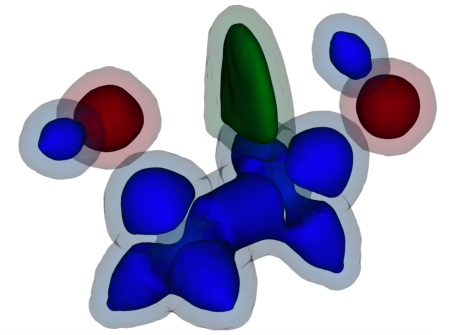
\includegraphics[width=\linewidth]{Images/EthaneDiol/fls_2_3.pdf}
\caption{$ZLS_{T}$ + $FLS_{T,2}$}
\label{}
\end{subfigure}
\begin{subfigure}{0.18\linewidth}
\centering
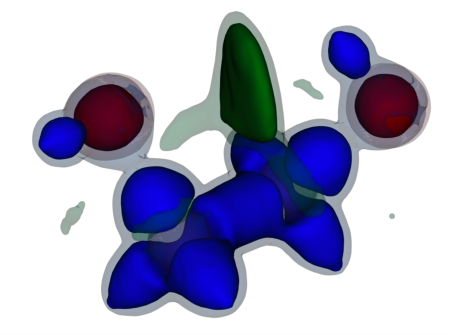
\includegraphics[width=\linewidth]{Images/EthaneDiol/fcls_68_3.pdf}
\caption{$ZLS_{T}$ + $FCLS_{T,68\%}$}
\label{}
\end{subfigure}
\begin{subfigure}{0.24\linewidth}
\centering
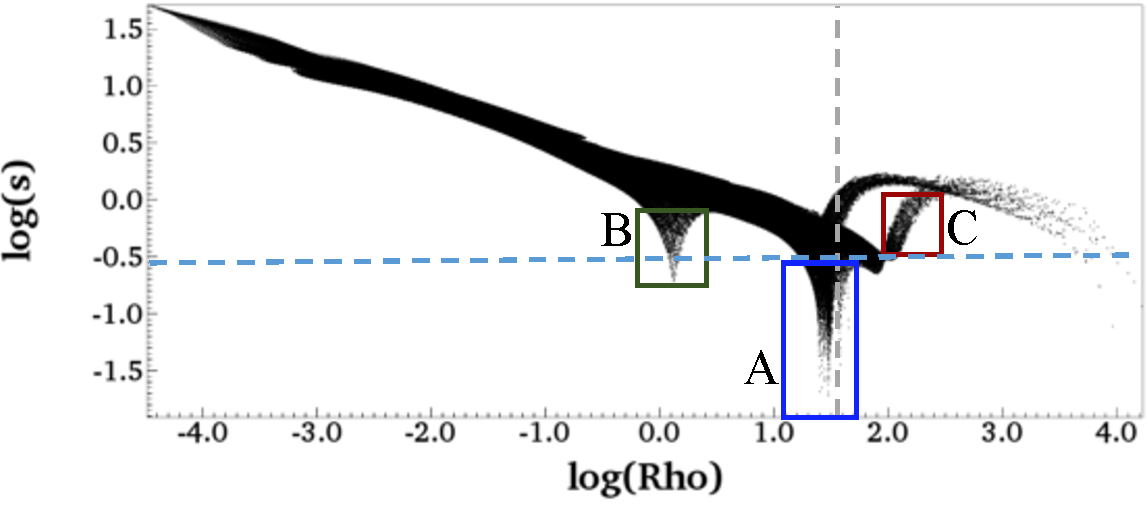
\includegraphics[width=\linewidth]{Images/EthaneDiol/scatterplot_3.pdf}
\caption{Attribute space 2D scatterplot, traits (labeled rectangular selections), and isovalues (dashed lines). We use $T = \left\{T_{A}, T_{B}, T_{C}\right\}$.} 
\label{}
\end{subfigure}
\caption{}
\label{}
\end{figure*}

\begin{figure*}[!h]
\begin{subfigure}{0.245\linewidth}
\centering
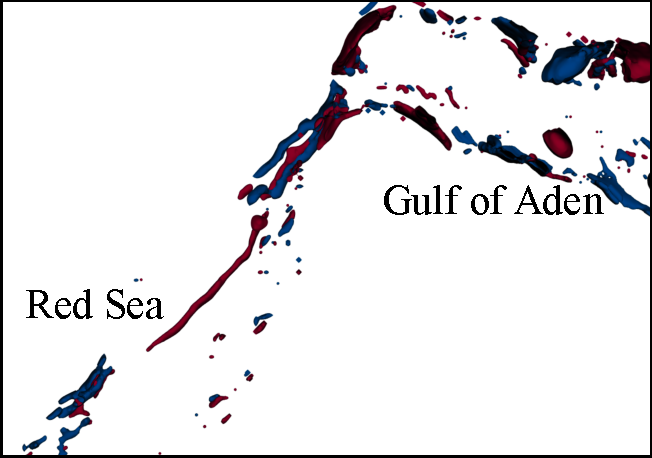
\includegraphics[width=\linewidth]{Images/RedSeaEddy/zls.pdf}
\vspace{-2mm}
\caption{$ZLS_{T}$}
\label{fig:rse_zls}
\end{subfigure}
\begin{subfigure}{0.245\linewidth}
\centering
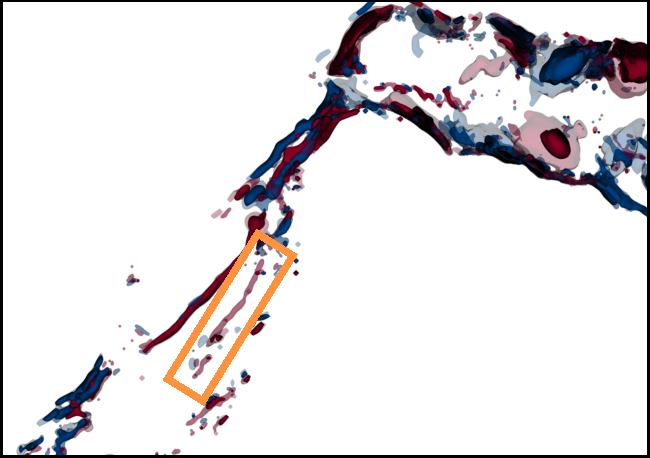
\includegraphics[width=\linewidth]{Images/RedSeaEddy/fcls_50.pdf}
\vspace{-2mm}
\caption{$ZLS_{T}$ + $FCLS_{T,50\%}$}
\label{fig:rse_fls}
\end{subfigure}
\begin{subfigure}{0.245\linewidth}
\centering
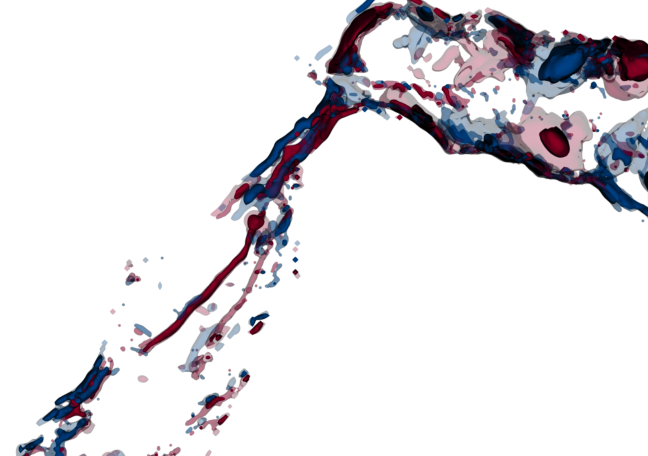
\includegraphics[width=\linewidth]{Images/RedSeaEddy/fcls_68.pdf}
\vspace{-2mm}
\caption{$ZLS_{T}$ + $FCLS_{T,68\%}$}
\label{fig:rse_fcls}
\end{subfigure}
\hfill
\begin{subfigure}{0.24\linewidth}
\centering
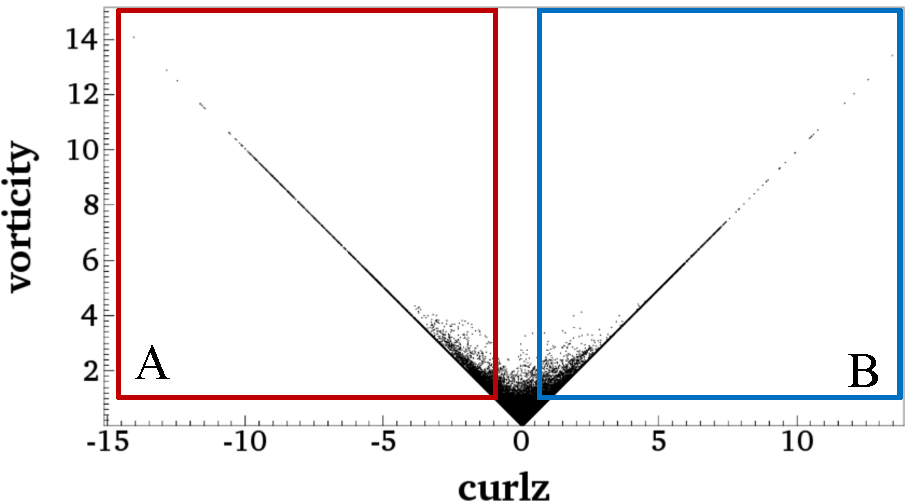
\includegraphics[width=0.95\linewidth]{Images/RedSeaEddy/scatterplot.pdf}
\vspace{-2mm}
\caption{Attribute space 2D scatterplot and traits (labeled rectangular selections). We use $T = \left\{T_{A}, T_{B}\right\}$.} 
\label{fig:rse_scatterplot}
\end{subfigure}
\vspace{-2mm}
\caption{Visualization of anticyclonic~($T_{A}$, red) and cyclonic~($T_{B}$, blue) eddies in the Gulf of Aden and part of the Red Sea using the derived attributes of vorticity magnitude and the z-component of curl. For this ensemble data set, $FCLS_{T,C}$ visualized additional paths and regions with eddies. The orange box in (c) highlights one such example.}
%\vspace{-1mm}
\label{fig:rse}
\end{figure*}

\begin{figure*}[!h]
\begin{subfigure}{0.2\linewidth}
\centering
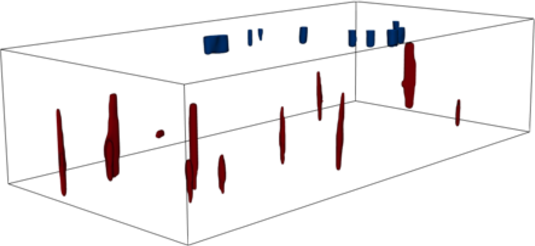
\includegraphics[width=\linewidth]{Images/Mantel/zls.pdf}
\vspace{-5mm}
\caption{$ZLS_{T}$}
\label{fig:mantel_zls}
\end{subfigure}
\begin{subfigure}{0.2\linewidth}
\centering
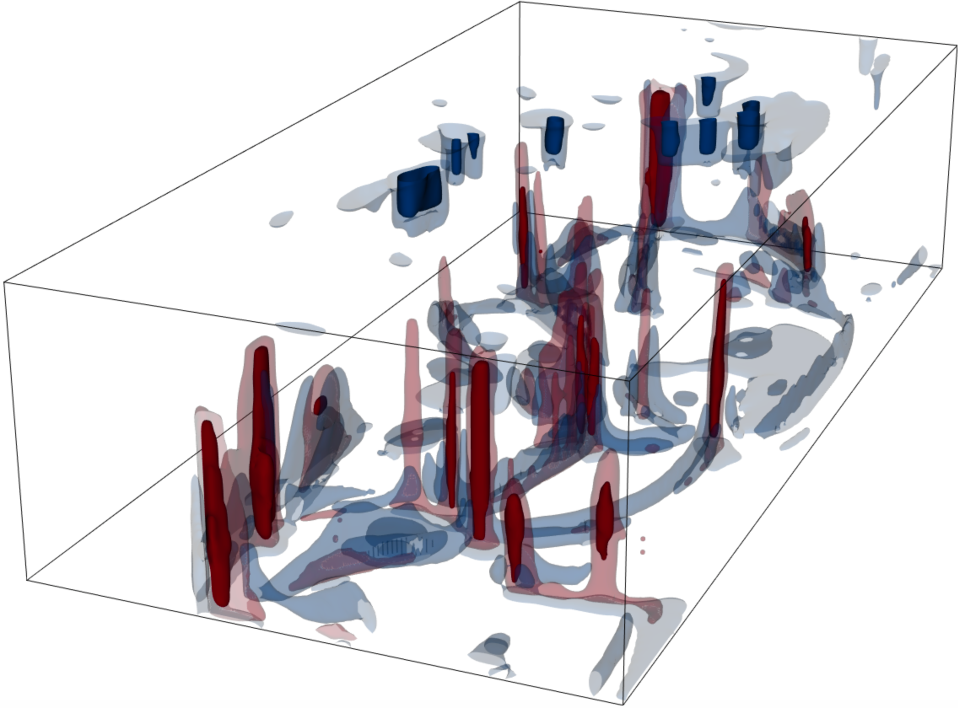
\includegraphics[width=\linewidth]{Images/Mantel/fcls_68.pdf}
\vspace{-5mm}
\caption{$ZLS_{T}$ + $FCLS_{T,68\%}$}
\label{fig:mantel_fls}
\end{subfigure}
\begin{subfigure}{0.295\linewidth}
\centering
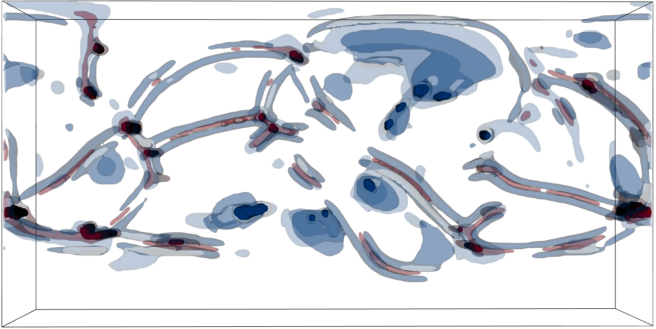
\includegraphics[width=0.9\linewidth]{Images/Mantel/fcls_68_v2.pdf}
\caption{$ZLS_{T}$ + $FCLS_{T,68\%}$}
\label{fig:mantel_fcls}
\end{subfigure}
\hfill
\begin{subfigure}{0.295\linewidth}
\centering
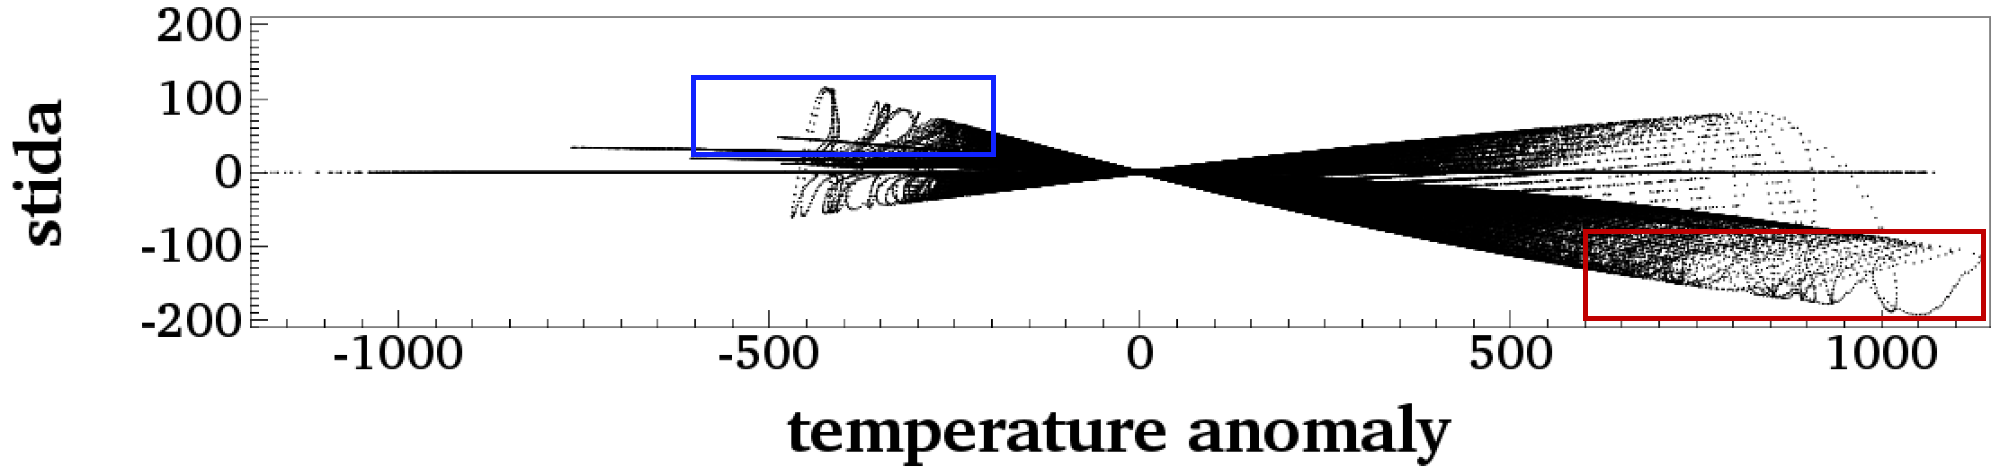
\includegraphics[width=\linewidth]{Images/Mantel/scatterplot.pdf}
%\vspace{-2mm}
\caption{Attribute space 2D scatterplot and traits (labeled rectangular selections). We use $T = \left\{T_{A}, T_{B}\right\}$.} 
\label{fig:mantel_scatterplot}
\end{subfigure}
\vspace{-2mm}
\caption{Visualization of rising hot plumes~($T_{A}$, red) and sinking material~($T_{B}$, blue) flow patterns in a subset of the spatial domain for the mantel data using the temperature anomaly and spin transition induced density anomaly~(stida) attributes.}
\label{fig:mantel}
\end{figure*}

